\section{Three Address Code}
FAC represents the three address code (3AC) using indirect triples. 
As stated by Aho et al. \cite{dragonbook}, this 
representation can help during the code optimization phase.
Indeed, the code optimizer can easily reorder the instructions without affecting
the triples themselves. We used a doubly-linked list instead of a single-linked
one to make it traversable in both directions.

FAC generates the 3AC by post-order traversing the AST filtered by the type checker. 

FAC uses \emph{only} synthesized attributes during the 3AC generation. 
This makes the whole process pretty easy to understand.

The 3AC representation of the example code \ref{f-code1} is depicted in 
Fig. \ref{fig:ind-trpl}.

\begin{figure}[H]
  \centering
  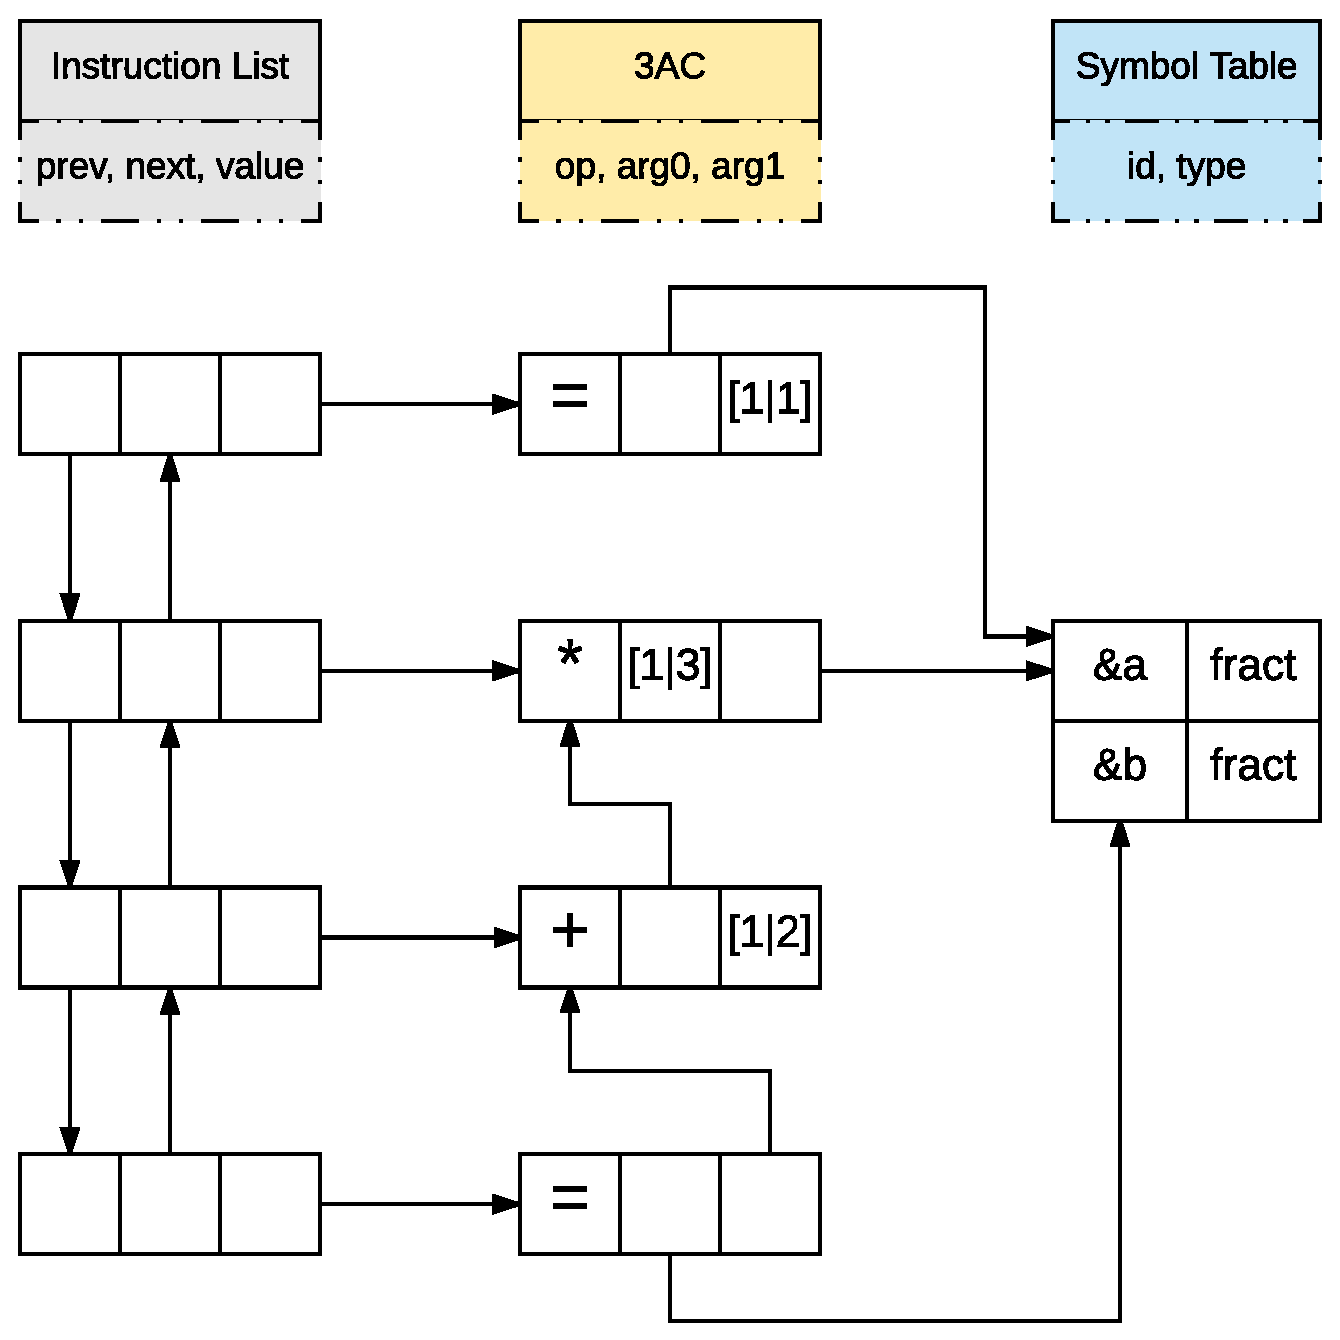
\includegraphics[width=.7\columnwidth]{img/eps/indirect_triples.eps}
  \caption{FAC - example of indirected triples.}
  \label{fig:ind-trpl}
\end{figure}
